\documentclass{article}
\usepackage{tikz}
\usetikzlibrary{matrix}

\begin{document}

\begin{figure}[h]
    \centering
    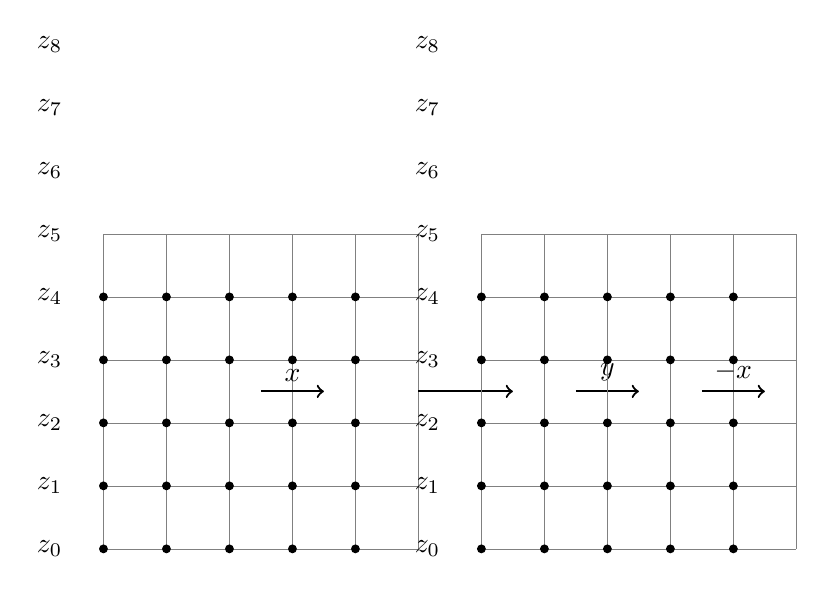
\begin{tikzpicture}[scale=0.8]
        % Grid for the first part
        \draw[help lines] (0,0) grid (5,5);
        
        % Labels for the rows
        \foreach \y [count=\i from 0] in {4,...,-4} {
            \node[left] at (-0.5,\i) {$z_{\i}$};
        }
        
        % Nodes for the grid
        \foreach \x in {0,...,4} {
            \foreach \y in {0,...,4} {
                \fill (\x,\y) circle (2pt);
            }
        }
        
        % Arrows and labels
        \draw[->, thick] (2.5,2.5) -- node[above] {$x$} (3.5,2.5);
        \draw[->, thick] (7.5,2.5) -- node[above] {$y$} (8.5,2.5);
        
        % Arrow between the two grids
        \draw[->, thick] (5,2.5) -- node[midway, above] {} (6.5,2.5);
        
        % Grid for the second part
        \draw[help lines] (6,0) grid (11,5);
        
        % Labels for the rows
        \foreach \y [count=\i from 0] in {4,...,-4} {
            \node[left] at (5.5,\i) {$z_{\i}$};
        }
        
        % Nodes for the grid
        \foreach \x in {0,...,4} {
            \foreach \y in {0,...,4} {
                \fill (\x+6,\y) circle (2pt);
            }
        }
        
        % Arrows and labels
        \draw[->, thick] (9.5,2.5) -- node[above] {$-x$} (10.5,2.5);
    \end{tikzpicture}
    \caption{A depiction of the transformation of the domain of the colored S6V model used in the proof of Lemma~\ref{l.S_N symmetry}. The $z_i$ labels at the left side indicate the spectral parameter for the colored S6V weights on the corresponding row.}
    \label{fig:S6V_domain_transformation}
\end{figure}

\end{document}